\section{La programmation orientée objet sous CodeSys}
\begin{UPSTIidee}{Application : Etape d'un grafcet}
    Afin de faciliter la compréhension de cette partie, nous allons construire, tout au long de ce cours, une classe \emph{CStep} qui représente une étape d'un grafcet. Cette classe contiendra les attributs et méthodes suivants :

    \begin{minipage}{.45\linewidth}
        \paragraph{Attributs}
        \begin{itemize}
            \item \textbf{m\_xActivityBit} : bit d'activité (actif ou non)
                  \begin{itemize}
                      \item Accessible en lecture uniquement
                  \end{itemize}
            \item \textbf{m\_tActivationDuration} : Stocke le temps d'activation de l'étape
                  \begin{itemize}
                      \item Accessible en lecture uniquement
                  \end{itemize}
            \item \textbf{m\_tTaskPeriod} : période de la tâche
                  \begin{itemize}
                      \item Accessible en lecture et en écriture
                  \end{itemize}
        \end{itemize}
    \end{minipage}%
    \begin{minipage}{.45\linewidth}
        \paragraph{Méthodes}
        \begin{itemize}
            \item \textbf{MInit} : Méthode appelée à l'initialisation du programme
            \item \textbf{MActivate} : active l'étape
            \item \textbf{MDeactivate} : désactive l'étape
        \end{itemize}
    \end{minipage}

\end{UPSTIidee}

\subsection{Les classes}
\label{subsec:classes}

On l'a vu, la notion de classe nous demande de pouvoir créer des attributs et des méthodes. Les attributs sont des variables internes aux classes qui devront être conservées entre deux utilisations d'un objet de cette classe.
L'utilisation de fonctions (POU FUNCTION) ne serait pas satisfaisante, car la durée de vie d'une variable interne à une fonction est limitée à l'exécution de cette fonction.

A l'inverse, un bloc fonctionnel s'utilise après en avoir créé une instance et ses variables internes sont conservées entre d'une utilisation à l'autre. Les POU FB semblent donc adaptées à la création de classes.

\UPSTIaRetenir{Nous utiliserons les blocs fonctions pour implémenter la notion de classe sous CodeSys.}

\begin{UPSTIinfor}{Déclaration d'une classe sous CodeSys}
    Définir une classe sous CodeSys revient à définir un bloc fonctionnel. Afin de différencier les variables privées (inaccessibles depuis l'extérieur) des attributs publics (accessibles depuis l'extérieur), on utilisera la convention suivante :
    \begin{itemize}
        \item Les variables publiques commenceront par \emph{m\_}
        \item les variables privées n'ont pas de préfixe particulier
    \end{itemize}

    Ainsi, la déclaration d'une classe \lstinline[language=ST]{<CName>} se fera de la manière suivante :
    \begin{lstlisting}
        FUNCTION_BLOCK <CName> (* définition de la classe <CName> *)
            VAR
                <type><Name> : <type>; (* variable locale non accessible de l'extérieur *)
                m_<type><Name> : <type>; (* membre de l'objet accessible de l'extérieur sous certaines conditions*)
            END_VAR
    \end{lstlisting}
\end{UPSTIinfor}

\begin{UPSTIidee}{Attributs de la classe CStep}
    Puisqu'elle ne possède que des attributs accessibles, la déclaration de notre classe \emph{CStep} se fera de la manière suivante :
    \begin{lstlisting}
FUNCTION_BLOCK FB_CStep
    VAR
        m_xActivityBit : BOOL; (* bit d'activité (actif ou non) *)
        m_tActivationDuration : TIME; (* Stocke le temps d'activation de l'étape *)
        m_tTaskPeriod : TIME; 
    END_VAR\end{lstlisting}

    L'instanciation d'un objet de cette classe pourra alors s'écrire \lstinline{Etape1 : FB_CStep;}

    Pour le moment, ces attributs ont été déclarés dans notre classe \emph{CStep} mais ils ne sont pas accessibles depuis l'extérieur (Il est impossible d'évaluer l'expression \lstinline{Etape1.m_xActivityBit}). Ces variables sont "coincées" à l'intérieur de notre bloc fonction. Pour les rendre accessibles, nous allons utiliser l'objet \lstinline{PROPERTY} proposé par CodeSys. 
\end{UPSTIidee}
\subsection{L'objet PROPERTY (propriété)}
\label{subsec:property}
L'objet \lstinline{PROPERTY} est un outil proposé par CodeSys pour la programmation orientée objet. Il permet de définir des attributs (variables) propres à un contexte avec un niveau d'accessibilité paramétrable (publique, privée, protégée ou interne).

Cela signifie que l'on peut définir des variables à l'intérieur d'une classe qui pourront être accessibles depuis l'extérieur de la classe par l'intermédiaire de méthodes appelées \emph{accesseurs}.

\begin{UPSTIinfor}{Les accesseurs}
    Il existe deux types d'accesseurs : GET et SET. 
    \begin{description}
        \item[GET] : Permet de lire la valeur d'une variable
        \item[SET] : Permet d'écrire la valeur d'une variable
    \end{description}
    \begin{minipage}{.45\linewidth}
        \begin{lstlisting}
            C<ClassName>.<propertyName>.Get 
                <propertyName> := THIS^.m_<localName>;
        \end{lstlisting}
    \end{minipage}%
    \hfill
    \begin{minipage}{.45\linewidth}
        \begin{lstlisting}
            C<ClassName>.<propertyName>.Set 
                THIS^.m_<localName> := <propertyName>;
        \end{lstlisting}
    \end{minipage}

    Il est possible de supprimer un des accesseurs pour rendre la propriété en lecture seule ou en écriture seule.

    Lors d'une dérivation, les propriétés de la classe sont héritées et leurs accesseurs peuvent être surchargés.
\end{UPSTIinfor}

Une propriété est donc un objet que l'on associe à une POU. On décrit ensuite ses accesseurs pour définir comment lire ou écrire la valeur de la propriété.
Ce sont elles qui permettent d'obtenir une encapsulation des données. En effet, elles permettent de contrôler l'accès aux données de l'objet (variables internes, d'un POU, d'un BF ou d'une variable globale -- GVL). Elles agissent comme un filtre ou une surchage. 


\begin{UPSTIinfor}{Ajout d'un propriété sous CodeSys}
    \begin{minipage}{.7\linewidth}
        Sous CodeSys, les propriétés et les méthodes sont ajoutés à la POU en utilisant l'outil \emph{Add Object}. Il suffit alors de sélectionner le type de l'objet à ajouter (propriété ou méthode) et de le nommer.
    \end{minipage}\hfill
    \begin{minipage}{.2\linewidth}
        \centering
        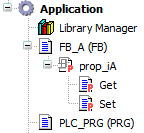
\includegraphics[width=\linewidth]{_cds_img_property.png}
    \end{minipage}    
\end{UPSTIinfor}

\begin{UPSTIidee}{Propriétés de la classe CStep}
    Par exemple, si notre classe \emph{CStep} possède un attribut \emph{m\_xActivityBit}, nous allons ajouter une propriété \emph{xActivityBit} à notre bloc fonctionnel \emph{FB\_CStep}. Cette propriété, en lecture seule, n'aura pas d'accesseur \emph{SET}. Son accesseur \emph{GET} sera défini de la manière suivante :
    \begin{lstlisting}
FB_CStep.xActivityBit.Get
    xActivityBit := THIS^.m_xActivityBit;
    \end{lstlisting}
\end{UPSTIidee}

\begin{UPSTIinfor}{Les attributs d'accessibilité}
    Les méthodes et les attributs sont associées à un attribut d'accessibilité. Cela permet de contrôler l'accès aux méthodes et aux attributs de la classe : 
    \begin{description}
        \item[PRIVATE] : Accessibilité réduite à l'entité à laquelle elle est associée.
        \item[PROTECTED] : Accessibilité réduite à l'entité à laquelle elle est associée et à ses dérivées.
        \item[PUBLIC] : Accessibilité à toutes les entités.
        \item[INTERNAL] : Accessibilité réduite à l'espace de noms de la bibliothèque
    \end{description}
\end{UPSTIinfor}

\subsection{Méthodes}
\label{subsec:methodes}
L'objet \lstinline{METHOD} est un outil proposé par CodeSys pour la programmation orientée objet. Il permet de définir des méthodes (fonctions) propres à un contexte avec un niveau d'accessibilité paramétrable (publique, privée, protégée ou interne).

Les avantages d'utiliser des méthodes au sein d'une classe sont les suivants : 
\begin{itemize}
    \item La modularité des blocs fonctionnels est favorisée
    \begin{itemize}
        \item On pourra décomposer le corps d'un bloc fonctionnel en plusieurs appels de méthodes
    \end{itemize}
    \item La lisibilité du code est améliorée
    \item l'intégrité des données est favorisée par l'utilisation judicieuse d'attributs d'accessibilité
\end{itemize}

Comme pour une fonction, on peut définir :
\begin{itemize}
    \item Des variables d'Entrées, de sorties ou d'entrées-sorties
    \item Des variables locales à la méthode
          \begin{itemize}
              \item La durée de vie de ces variables locales est alors limitée à l'exécution de la méthode
          \end{itemize}
\end{itemize}

Par ailleurs, \textbf{une méthode a accès au contexte de l'instance à laquelle elle est associée}. Cela signifie qu'elle a accès aux variables et méthodes de l'objet dont elle dépend.

Enfin, CodeSys autorise la déclaration de \lstinline{METHOD}s dans une interface. Elle devra alors être implémentée dans les classes qui implémentent cette interface.

\UPSTIaRetenir{Les méthodes des classes que nous définirons seront des méthodes associées au bloc fonction concerné.

Leur ligne de déclaration est la suivante : \lstinline{METHOD <Attribut> <Method_Name> | : <return_data_type>}}

\begin{UPSTIidee}{Les méthodes de la classe CStep}
        \begin{minipage}[t]{.6\linewidth}
            Les méthodes de la classe \emph{CStep} seront définies dans le bloc fonctionnel \emph{FB\_CStep}. Elles seront donc des méthodes associées à ce bloc fonctionnel.
        \paragraph{Méthodes}
        \begin{itemize}
            \item \textbf{MInit} : Méthode appelée à l'initialisation du programme
            \item \textbf{MActivate} : active l'étape
            \item \textbf{MDeactivate} : désactive l'étape
        \end{itemize}
    \end{minipage}%
    \begin{minipage}[t]{.35\linewidth}
        \begin{lstlisting}
METHOD PUBLIC MInit : BOOL
    VAR_INPUT
    END_VAR
    VAR_OUTPUT
    END_VAR
    VAR
    END_VAR
    // Code de la méthode
    // ...
    // Fin du code de la méthode
END_METHOD
        \end{lstlisting}
    \end{minipage}
\end{UPSTIidee}
\subsection{Les interfaces}
\label{subsec:interfaces}
Une interface est un ensemble de méthodes et de propriétés qui définissent un contrat. Une classe qui implémente une interface doit alors implémenter toutes les méthodes et propriétés de cette interface. Cela permet de définir une structure très générique qui sera utilisée, ensuite, par les classes que nous définirons. 

\UPSTIaRetenir{Les interfaces permettent de définir un contrat que les classes qui les implémentent doivent respecter. La déclaration d'une interface se fait de manière similaire à la déclaration d'une classe, mais aucune méthode n'est implémentée.}
\lstDeleteShortInline~
\begin{UPSTIactivite}[][Exemple d'interface]
    \UPSTIquestion{Donner un exemple dans lequel l'utilisation d'une interface est pertinente, par exemple dans le monde du jeu vidéo. Expliquer}
    \vspace{5cm}
\end{UPSTIactivite}

\begin{UPSTIinfor}{Les interfaces sous CodeSys}
    \begin{minipage}{.7\linewidth}
        Sous CodeSys, une interface s'ajoute dans l'arborescence du projet en utilisant l'outil \emph{Add Object}. Il suffit alors de sélectionner le type de l'objet à ajouter (interface) et de le nommer. Elle apparaît alors ainsi que les méthodes et propriétés qui lui sont associées. 
        
        Le mot clef utilisé sous CodeSys est \lstinline{INTERFACE}.


        Le mot clef \lstinline{IMPLEMENT} est utilisé lors de la déclaration d'une classe pour indiquer que cette classe implémente une interface.


        
    \end{minipage}
    \hfill
    \begin{minipage}{.25\linewidth}
        \centering
        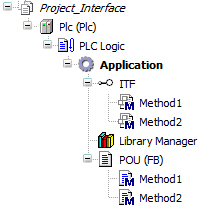
\includegraphics[width=\linewidth]{_cds_img_itf_method.png}
    \end{minipage}

\end{UPSTIinfor}

\paragraph{Dans notre contexte} les interfaces pourront définir, pour un ensemble de blocs fonctionnels : 
\begin{itemize}
    \item Des propriétés (\lstinline{PROPERTY})
    \begin{itemize}
        \item Nom
        \item Type
        \item Accesseurs
    \end{itemize}
    \item Des méthodes (\lstinline{METHOD})
    \begin{itemize}
        \item Nom
        \item Paramètres d'entrées et de sorties (\lstinline{VAR_INPUT}, \lstinline{VAR_OUTPUT}, \lstinline{VAR_IN_OUT})
    \end{itemize}
\end{itemize}

\begin{UPSTIinfor}{Plusieurs interfaces}
    Une classe peut implémenter plusieurs interfaces. Elle devra alors implémenter toutes les méthodes et propriétés de ces interfaces.

    \begin{lstlisting}
FUNCTION_BLOCK <fb_name> IMPLEMENTS <ITF_name_0> |, <ITF_name_1> |, <ITF_name_n>
    \end{lstlisting}
\end{UPSTIinfor}

%%% TODO : Ajouter les interfaces comme groupe homogène (slides 13-14) %%%
\subsection{Les pointeurs spéciaux}
\label{subsec:pointeurs_speciaux}
CodeSys défini deux vecteurs spéciaux \lstinline{THIS} et \lstinline{SUPER}. Leur utilisation est réservée au contexte de la POO, dans le corps d'un bloc fonctionnel ou dans les méthodes associées.
\subsubsection{le pointeur THIS} 

Le pointeur \lstinline{THIS} est un pointeur spécial qui pointe vers l'objet auquel appartient la méthode. Il est automatiquement disponible dans tous les blocs fonctions. 

Les utilisations principales de \lstinline{THIS} sont données ci-dessous, les exemples sont extraits de la documentation en ligne de CodeSys. 

\paragraph{Démasquage d'une propriété ou d'une méthode : } Par exemple, lorsqu'une variable locale a le même nom qu'une propriété de l'objet, il est nécessaire de démasquer l'objet pour accéder à la propriété.  

\lstinputlisting[multicols=2]{this_exemple1.st}

\paragraph{Désigner l'objet tout entier} lors d'un passage d'objet en paramètre d'une méthode.

\lstinputlisting[multicols=2]{this_exemple2.st}

\subsubsection{Le pointeur SUPER}
Le pointeur \lstinline{SUPER} est un pointeur spécial qui pointe vers l'objet parent de l'objet auquel appartient la méthode. Il est automatiquement disponible dans tous les blocs fonctions. Par définition, son utilisation est réservée aux blocs fonctionnels obtenus par dérivation. 

Ce pointeur permet d'accéder aux méthodes et propriétés de l'objet parent, notamment quand celles-ci ont été surchargées dans les blocs fonctionnels dérivés. 

Le code suivant, issu de la documentation en ligne de CodeSys, montre quelques exemples d'utilisation des pointeurs \lstinline{SUPER} et \lstinline{THIS}.

\lstinputlisting[multicols=2]{super_exemple.st}
\subsection{Construction des objets}
\label{subsec:construction_objets}
La construction d'un objet consiste à lui donner des valeurs spécifiques d'initialisation pour chacun de ses membres. Lors de l'instanciation d'un bloc fonction, CodeSys appelle automatiquement, et en premier lieu, la méthode \lstinline{FBInit} de l'objet. Cette méthode est créée implicitement et peut être surchargée pour définir une initialisation particulière. 

Son protoype est le suivant : 
\begin{lstlisting}
METHOD FB_Init : BOOL
VAR _INPUT
    bInitRetains : BOOL;
    bInCopyCode : BOOL;
END_VAR
\end{lstlisting}

\UPSTIaRetenir{\begin{itemize}
    \item La méthode \lstinline{FBInit} est définie implicitement lors de la déclaration d'un bloc fonction.
    \item Elle peut être surchargée pour définir une initialisation particulière.
    \item Elle est appelée la première et automatiquement lors de l'instanciation d'un bloc fonction.
    \end{itemize}}




\subsection{Mise en oeuvre}
Cette section propose un exemple de mise en oeuvre de la programmation orientée objet sous CodeSys. Nous allons construire une classe \emph{CStep} qui représente une étape d'un grafcet. Cette classe implémentera une interface \emph{ITF\_ObjStep} qui définira les méthodes et attributs communs à toutes les étapes : 
\begin{itemize}
    \item \textbf{Attributs}
          \begin{itemize}
              \item \textbf{m\_xActivityBit} : bit d'activité (actif ou non)
                    \begin{itemize}
                        \item Accessible en lecture uniquement
                    \end{itemize}
              \item \textbf{m\_tActivationDuration} : Stocke le temps d'activation de l'étape
                    \begin{itemize}
                        \item Accessible en lecture uniquement
                    \end{itemize}
              \item \textbf{m\_tTaskPeriod} : période de la tâche
                    \begin{itemize}
                        \item Accessible en lecture et en écriture
                    \end{itemize}
          \end{itemize}
    \item \textbf{Méthodes}
    \begin{itemize}
        \item \textbf{MInit} : Méthode appelée à l'initialisation du programme
        \item \textbf{MActivate} : active l'étape
        \item \textbf{MDeactivate} : désactive l'étape
    \end{itemize}
\end{itemize}

\begin{UPSTIactivite}[][L'interface \lstinline{ITF_ObjStep}]
\UPSTIquestion{Compléter la liste des propriété et méthodes de l'interface \lstinline{ITF_ObjStep}.}

\begin{lstlisting}[escapechar=~, numbers=none, basicstyle=\Large, language=st]
~
\includegraphics[height=\fontcharht\font`\B]{_cds_icon_interface.png}~INTERFACE ITF_ObjStep
    ~
\includegraphics[height=\fontcharht\font`\B]{_cds_icon_interface_property.png}~ PROPERTY xActivityBit : BOOL (*Accesseur Get*)
    ~
\includegraphics[height=\fontcharht\font`\B]{_cds_icon_interface_property.png}~ PROPERTY ~\dotfill~
    ~
\includegraphics[height=\fontcharht\font`\B]{_cds_icon_interface_property.png}~ PROPERTY ~\dotfill~
    ~$\cdots$~
    ~
\includegraphics[height=\fontcharht\font`\B]{_cds_icon_method.png}~ METHOD MInit;
    ~
\includegraphics[height=\fontcharht\font`\B]{_cds_icon_method.png}~ METHOD ~\dotfill~
    ~
\includegraphics[height=\fontcharht\font`\B]{_cds_icon_method.png}~ METHOD ~\dotfill~
\end{lstlisting}
\end{UPSTIactivite}
\pagebreak
\begin{UPSTIactivite}[][Le bloc fonction \lstinline{CStep}]
\UPSTIquestion{Compléter la déclaration du bloc fonctionnel \lstinline{CStep} qui implémente l'interface \lstinline{ITF_ObjStep}. Elle contiendra les variables locales associées aux propriétés de l'interface.}
\begin{lstlisting}[escapechar=~, basicstyle=\Large, language=st]
FUNCTION_BLOCK ~\dotfill~
VAR
    ~\dotfill~
    ~\dotfill~
    ~\dotfill~
END_VAR
\end{lstlisting}
\UPSTIquestion{Ajouter des lignes permettant la mise à jour de la durée d'activation lorsque l'étape est active -- Si l'étape est active, la durée d'activation augmente de la période de la tâche.}
\begin{lstlisting}[escapechar=~, basicstyle=\Large, language=st]
~\dotfill~
~\dotfill~
~\dotfill~
~\dotfill~
\end{lstlisting}
\UPSTIquestion{Définir les accesseurs pour les propriétés de l'interface.}
\begin{lstlisting}[numbers=none, escapechar=~, basicstyle=\Large, language=st]
~
\includegraphics[height=\fontcharht\font`\B]{_cds_icon_interface_property.png}~CStep.xActivityBit.Get
    ~\dotfill~
~
\includegraphics[height=\fontcharht\font`\B]{_cds_icon_interface_property.png}~CStep~\dotfill~
    ~\dotfill~
~
\includegraphics[height=\fontcharht\font`\B]{_cds_icon_interface_property.png}~CStep~\dotfill~
    ~\dotfill~
~
\includegraphics[height=\fontcharht\font`\B]{_cds_icon_interface_property.png}~CStep.Set (*Limiter les valeurs admissible a [T#1ms, T#10s]*)
    ~\dotfill~
    ~\dotfill~
    ~\dotfill~
    ~\dotfill~
\end{lstlisting}
\end{UPSTIactivite}
\pagebreak
\begin{UPSTIactivite}
    \UPSTIquestion{Surcharger le constructeur de la classe \lstinline{CStep} pour initialiser la période de la tâche à \lstinline{T#1ms}, le bit d'activité à \lstinline{FALSE} et la durée d'activation à \lstinline{T#0s}.}
    \begin{lstlisting}[numbers=none, escapechar=~, basicstyle=\Large, language=st]
~
\includegraphics[height=\fontcharht\font`\B]{_cds_icon_method.png}~METHOD~\dotfill~
    ~\dotfill~
    ~\dotfill~
    ~\dotfill~
    ~\dotfill~
    ~\dotfill~
    ~\dotfill~
    ~\dotfill~
    ~\dotfill~
    ~\dotfill~
\end{lstlisting}
\end{UPSTIactivite}
\begin{UPSTIactivite}
    \UPSTIquestion{Définir les méthodes \lstinline{MInit}, \lstinline{MActivate} et \lstinline{MDeactivate} de la classe \lstinline{CStep}.}
    \begin{lstlisting}[numbers=none, escapechar=~, basicstyle=\Large, language=st]
~
\includegraphics[height=\fontcharht\font`\B]{_cds_icon_method.png}~METHOD CStep.MInit 
    ~\dotfill~
    ~\dotfill~
    ~\dotfill~
~
\includegraphics[height=\fontcharht\font`\B]{_cds_icon_method.png}~METHOD CStep.MActivate 
    ~\dotfill~
    ~\dotfill~
    ~\dotfill~
    ~\dotfill~
    ~\dotfill~
~
\includegraphics[height=\fontcharht\font`\B]{_cds_icon_method.png}~METHOD CStep.MDeactivate
    ~\dotfill~
    \end{lstlisting}
\end{UPSTIactivite}

\pagebreak
\begin{UPSTIactivite}[][Utilisation]
    \UPSTIquestion{Compléter le programme suivant pour utiliser la classe \lstinline{CStep}. Le programme activera l'étape au premier cycle et la désactivera au bout de \SI{30}{\second}.}
    \lstinputlisting[numbers=none, escapechar=~, basicstyle=\Large, language=st]{usercase.st}
\end{UPSTIactivite}








